\documentclass[12pt,a4paper]{article}

%% Sets page size and margins
\usepackage[a4paper,top=2cm,bottom=2cm,left=1.5cm,right=1.5cm,marginparwidth=1.75cm]{geometry}

%% Language and font encodings
\usepackage[english]{babel}
\usepackage[utf8x]{inputenc}
\usepackage[T1]{fontenc}
\usepackage{subfig}

\usepackage[normalem]{ulem}
\useunder{\uline}{\ul}{}

%% Useful packages
\usepackage{graphicx}
\usepackage[colorinlistoftodos]{todonotes}
\usepackage[colorlinks=true, allcolors=black]{hyperref}
\usepackage[section]{placeins}
\usepackage{parskip}
\usepackage{natbib}
\usepackage{mathtools}
\usepackage{tikz}
\usepackage{subfig}
\usepackage{amsmath}
\usepackage{algorithm}
\usepackage[noend]{algpseudocode}
\usepackage{capt-of}

\usepackage{fancyhdr}
\pagestyle{fancy}
\fancypagestyle{plain}{
\lhead{ContempoaryComputerScience/NetworkAnalysis/Assignment2019}
	%Assignment 2019}
%\rhead{Anonymous Marking Code: Z0974445}
\rhead{Oliver Baxandall - htdv92}
\cfoot{\thepage}
\renewcommand{\headrulewidth}{0.4pt}
\renewcommand{\footrulewidth}{0.4pt}
}
\pagestyle{plain}% Set page style to plain.

%\setlength{\parskip}{10pt}%

\title{Network Analysis Assignment}
\date{}

\begin{document}
\maketitle
\section{Question 1: Ring Group Graphs}
\subsection{Degree Distribution}
Initially, we analyse the degree distribution of Ring Group Graphs. Analysis will  focus on how varying the values of p and q affect degree distribution for fixed values of m and k. By default, graphs depicting degree distribution are averaged over 100 samples.

The values p and q are constrained linearly. In order for clear comparison, when graphically displaying results, plots will be coloured according to figure \ref{legend}. High values of p with lower q are coloured red and vice versa comparisons are yellow.

 \begin{figure*}[h]
	\centering
	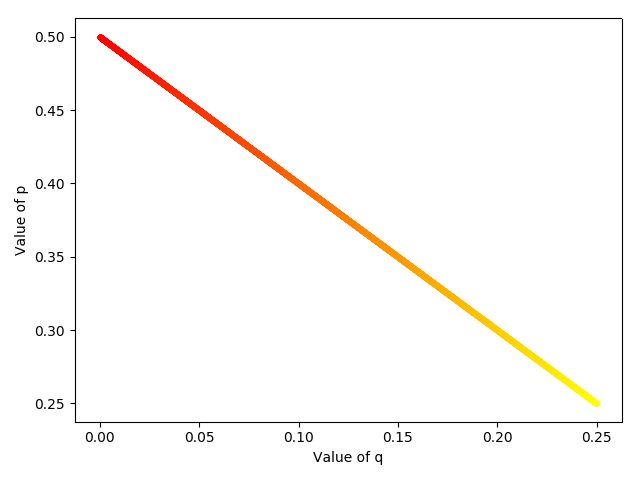
\includegraphics[width=10cm]{Figures/1/Legend.png}
	\caption{Colour indications of values for p and q under the constrains: p+q=0.5 p>q}
	\label{legend}
\end{figure*}

The Expected degree of each vertex in a ring group graph is as follows:

\begin{align*}
	Expected(Degree) =  p[(k-1) + 2k] + q[k(m-3)] = p[3k-1] + q[mk-3k)]
\end{align*} 

For a vertex, v, there are (k-1) other vertices in its group followed by 2k vertices in adjacent groups. v has probability p in having an edge between each of these vertices and so will be connected to approximately p[3k-1] vertices from this group. There are (m-3) other groups to choose from each with k vertices, with an edge  between v and each of these vertices forming with probability q, giving q[mk-3k)]. The degree distribution for a given graph should therefore average around this result.

Figure 2(a) approximates the degree distribution to that of a normal distribution, plotted from the mean and variance. The similarity between the plots shows that the degree distribution follows a normal trend, a property shared amongst all ring group graphs independent of the parameters. The distribution is technically binomial, as degree distribution is discrete data, indicated by an aggregated probability of a vertex connecting to any other vertex, averaged over all vertices. For the purposes of analysis, the binomial distribution will be approximated to normal, given that the sample size is sufficiently large. A black line is presented on all normalized results, indicating the normal approximation for each plot.

\begin{figure*}
	\centering
	\subfloat[m=100 k=100]{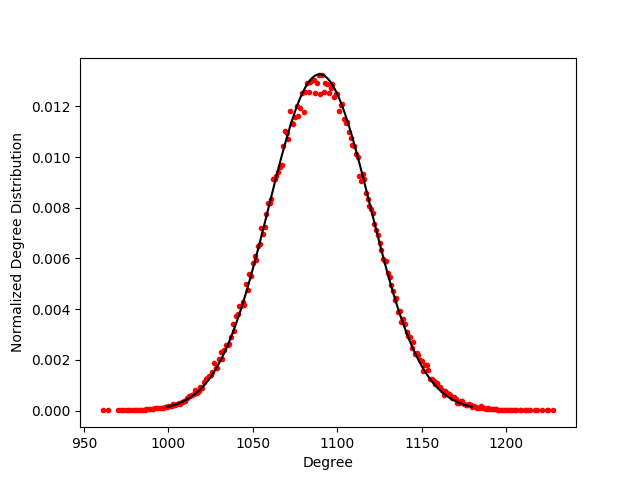
\includegraphics[width=8.4cm,height=6cm]{Figures/1/Distribution/m100k100.png}}
	\qquad
	\subfloat[m=100 k=100]{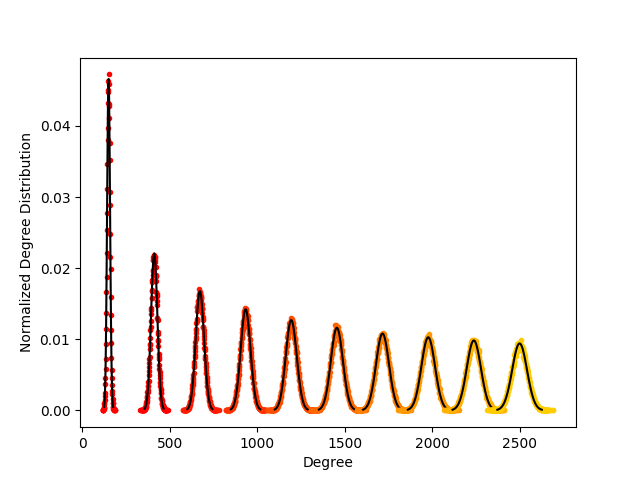
\includegraphics[width=8.4cm,height=6cm]{Figures/1/Distribution/m100k100group.png}}
	\caption{Degree Distribution Plots for two ring group graphs, holding m and k constant}
	\label{both}
\end{figure*}


\begin{table}[]
	\centering
	\caption{m = 100, k = 100}
	\begin{tabular}{|c|c|c|c|c|c|}
		\hline
		{\ul \textbf{p}} & {\ul \textbf{q}} & {\ul \textbf{Mean}} & {\ul \textbf{Variance}} & {\ul \textbf{Range}} & {\ul \textbf{Number Of Edges}} \\ \hline
		\textbf{0.5}     & \textbf{0.0}     & 149.527            & 74.019                  & 60                   & 747673                       \\ \hline
		\textbf{0.472}   & \textbf{0.028}   &  40.487           &  330.025                & 118                   & 2052458                     \\ \hline
		\textbf{0.444}   & \textbf{0.056}   &  671.833            & 563.938               & 166                   & 3359116                     \\ \hline
		\textbf{0.417}   & \textbf{0.083}   & 932.701            & 787.185            & 184                   & 4663562                      \\ \hline
		\textbf{0.389}   & \textbf{0.111}   & 1194.018           & 989.908               & 204                   & 5970297                    \\ \hline
		\textbf{0.361}   & \textbf{0.139}   & 1455.129           & 1182.969                & 219                  &7275389                     \\ \hline
		\textbf{0.333}   & \textbf{0.167}   & 1716.392            & 1356.899                &  237                 &8582159                      \\ \hline
		\textbf{0.306}   & \textbf{0.194}   & 1977.462			  & 1524.882                & 245                   & 9887613                   \\ \hline
		\textbf{0278}    & \textbf{0.222}   & 2238.786           &  1646.596                & 254                  & 11193790                      \\ \hline
		\textbf{0.25}    & \textbf{0.25}    & 2500             & 1784.87                & 268                  &12496676                      \\ \hline
	\end{tabular}
\end{table}


Figure 2(b) and table 1 shows how varying q from 0 to 0.25 and subsequently p respectively, impacts the degree distribution. The general trend following a normal distribution does not change, however the mean and variance do. Increasing q leads to larger degree variation per vertex as the height of each plot shrinks as the tails move further apart. 

As q increases, so does the total number of edges and the variance, as can be seen in table 1. This is because as the p and q get closer together, the ring group graph is more similar to a random graph, doing so completely when p=q=0.25. When p is higher, the vertices dominant method for connecting edges to other vertices is doing so with probability p between those in the same and adjacent groups. The number of nodes then to connect to with probability p is less than that for probability q. Therefore, degrees tend to be distributed less at higher p values where connections with probability p dominate over few vertices. This explains why the plots become shorter and fatter as p decreases relative to q. The table explains this well, showing the increasing number of edges are q increases with the growing variance and mean degree.

\begin{figure*}[]
	\centering
	\subfloat[m=50 k=50]{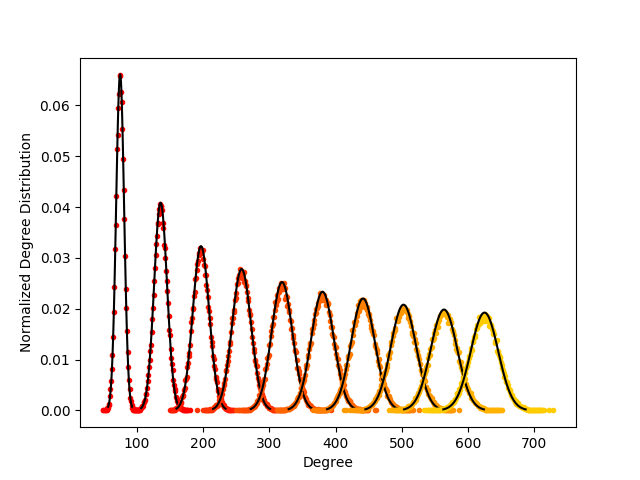
\includegraphics[width=8.4cm, height=6cm]{Figures/1/Distribution/m50k50.png}}
	\qquad
	\subfloat[m=10 k=10]{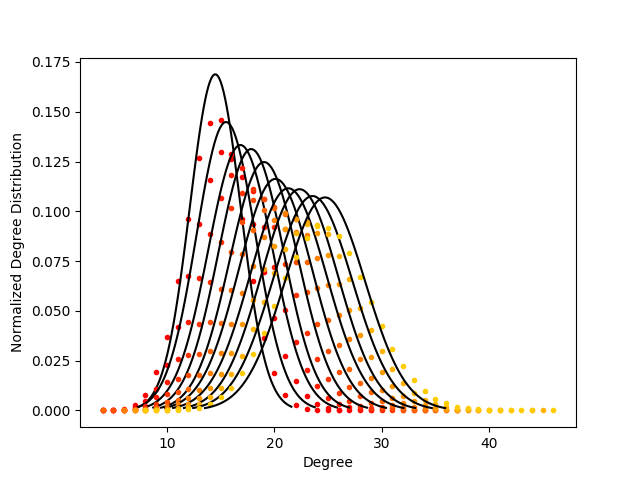
\includegraphics[width=8.4cm, height= 6cm]{Figures/1/Distribution/m10k10.png}}
	\caption{Ring Group Graph for m=k}
	\label{both}
\end{figure*}

\begin{figure*}[]
	\centering
	\subfloat[m=100 k=50]{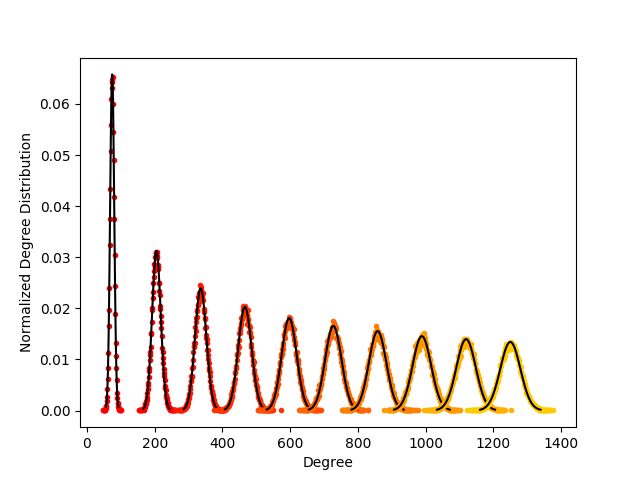
\includegraphics[width=8.4cm, height=6cm]{Figures/1/Distribution/m100k50.png}}
	\qquad
	\subfloat[m=50 k=100]{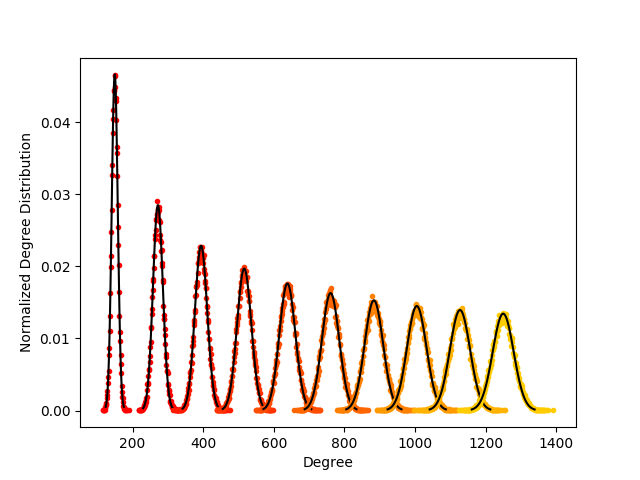
\includegraphics[width=8.4cm, height= 6cm]{Figures/1/Distribution/m50k100.png}}
	\caption{Ring Group Graph for values 50 and 100 for m and k respectively}
	\label{both}
\end{figure*}

\begin{figure*}[]
	\centering
	\subfloat[m=100 k=10]{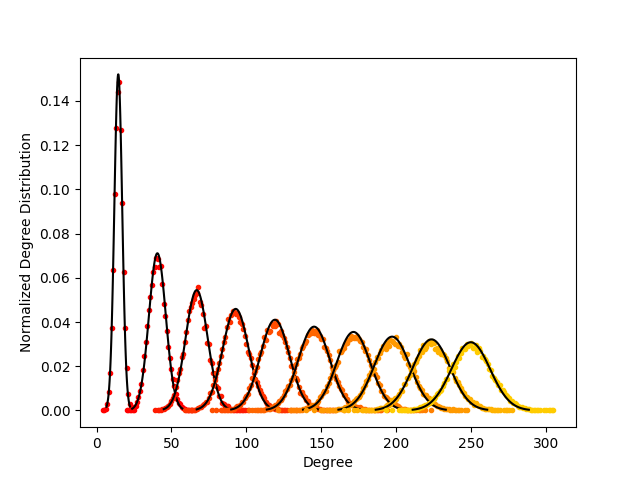
\includegraphics[width=8.4cm, height=6cm]{Figures/1/Distribution/m100k10.png}}
	\qquad
	\subfloat[m=10 k=100]{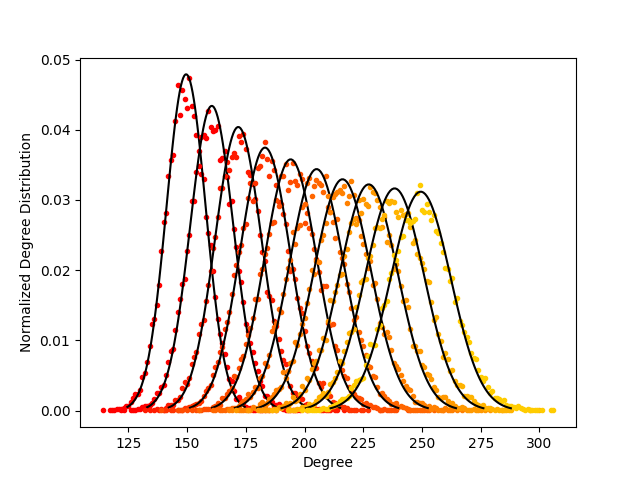
\includegraphics[width=8.4cm, height= 6cm]{Figures/1/Distribution/m10k100.png}}
	\caption{Ring Group Graph for values 10 and 100 for m and k respectively}
	\label{both}
\end{figure*}

\begin{figure*}[]
	\centering
	\subfloat[m=100 k=2]{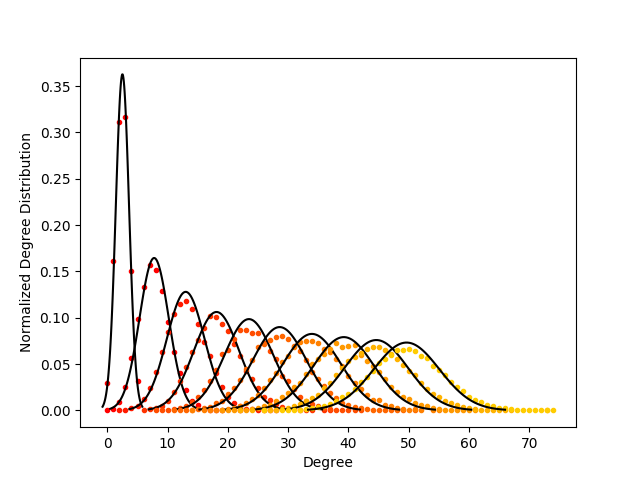
\includegraphics[width=8.4cm, height=6cm]{Figures/1/Distribution/m100k2.png}}
	\qquad
	\subfloat[m=2 k=100]{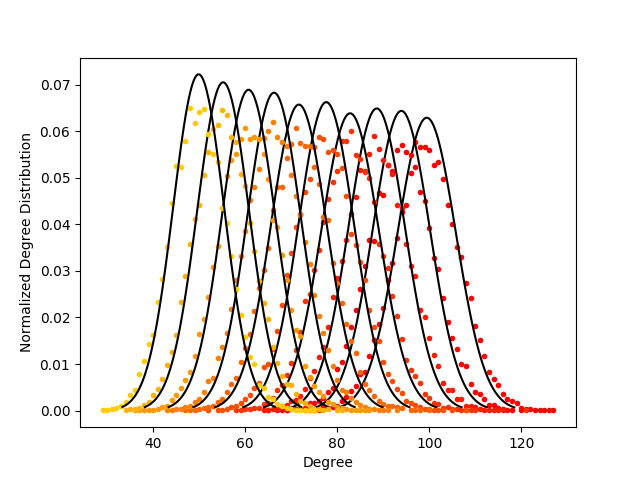
\includegraphics[width=8.4cm, height= 6cm]{Figures/1/Distribution/m2k100.png}}
	\caption{Ring Group Graph for values 2 and 100 for m and k respectively}
	\label{both}
\end{figure*}

Figures 3 to 6 show how the relationship changes for different values of m and k. Figure 3 continues from figure 2, showing distributions over values m=k. For the others, the left-hand side indicates graphs when m > k and the right m < k.

All of the figures verify the conclusions drawn from figure 2(b) in the increasing variance as q increases, although at different rates. If m > k, it can be seen that the process happens at a more immediate rate in comparison to where m < k where the height reduction and variance increase is less apparent. This is because for low values of m and k, the ring group property of the graphs stops holding and the graph becomes a closer representation of a random graph. When m < k, more vertices are being connected with probability p within their own group and for m > k, vertices are connected outside to others with probability q, as fewer vertices exist in their group. Since p > q, the relative decline in each graph is a reflection of which probability the graph is depending on more.  


\newpage
\subsection{Diameter}
Analysing the relationship between the value of p and the diameter for RG graphs for a fixed value of q. Figures 7 and 8 shows the plots created under these conditions, averaged over 10 samples because calculating the diameter is computationally time consuming. Diameter is a measure of connectivity in an undirected graph. A graph with a higher degree distribution therefore is more likely to have a smaller diameter. 

As can be seen, for values of q greater than approximately 0.15, the diameter of the graph is consistently 2. q is a measure of connectivity between groups in a ring group graph and so as it increases, movement between groups is better facilitated and as such the diameter is likely to fall. p measures connectivity inside of groups and is thus not as significant towards calculating the diameter. However, viewing it as non-deterministically pick a neighbour from a vertex, which is connected to a target vertex (or switching the vertices round) highlights why p still holds significance. Having a high value of p spreads out the value of q over more of the vertices in a group and so allows one vertex in a group to move to any other group by simply moving to a neighbour that is connected to it.

This can be seen effectively in figure 7 and 8, which shows the diameter reaching its lowest value when q is above 0.2 very any values of p, then slowly moving to a degree of 3 when q is 0.05 and then increasing exponentially as q decreases towards 0.
\begin{figure*}[h]
	\centering
	\subfloat[q = 0.0]{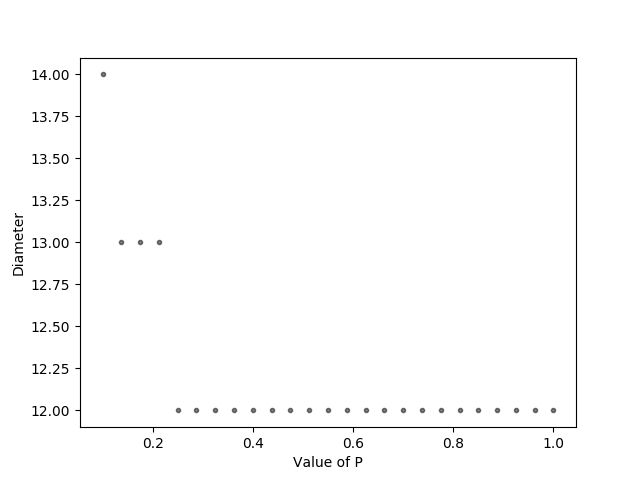
\includegraphics[width=8.4cm]{Figures/1/Diameter/m25k25num25q0.png}}
	\qquad
	\subfloat[q = 0.01]{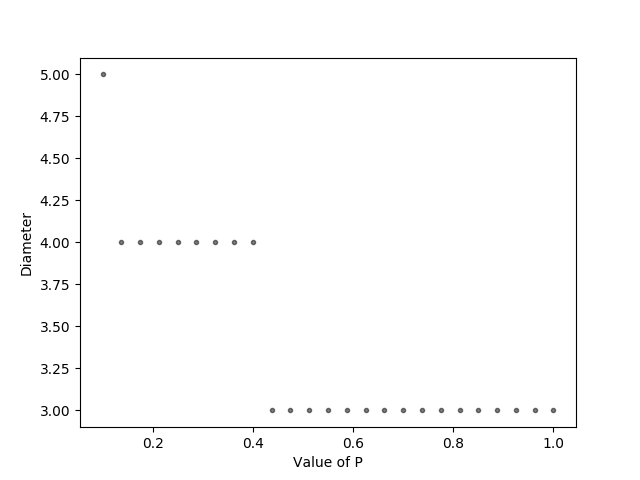
\includegraphics[width=8.4cm]{Figures/1/Diameter/m25k25num25q001.png}}
	\caption{The Diameter when varying p in a Ring Group graph for fixed q: part1}
	\label{diameters}
\end{figure*}

\begin{figure*}[h]
	\centering
	\subfloat[q = 0.05]{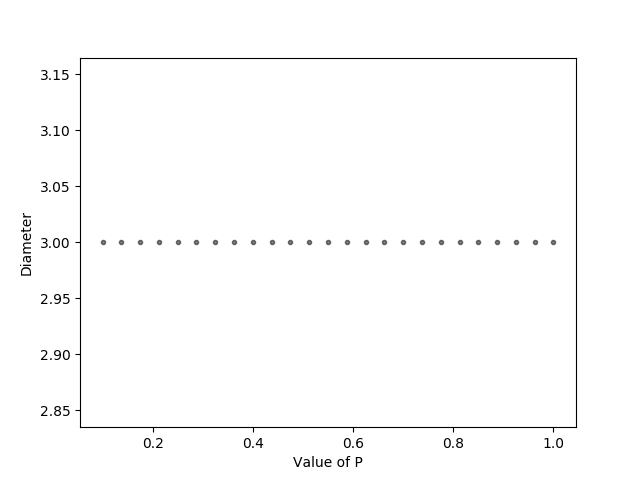
\includegraphics[width=8.4cm]{Figures/1/Diameter/m25k25num25q05.png}}
	\qquad
	\subfloat[q = 0.1]{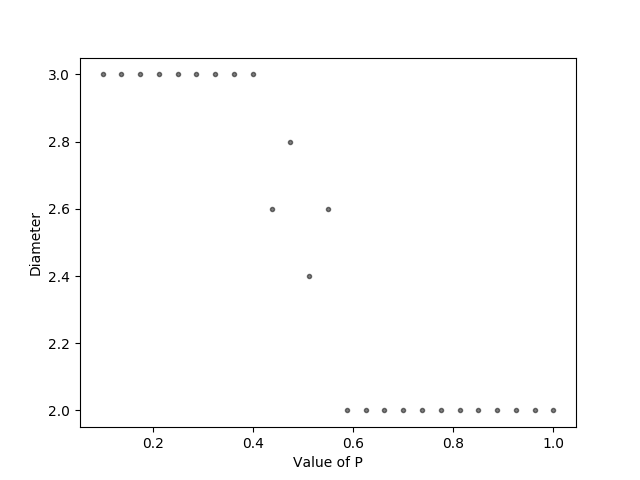
\includegraphics[width=8.4cm]{Figures/1/Diameter/m25k25num25q1.png}}
	\qquad
	\subfloat[q = 0.15]{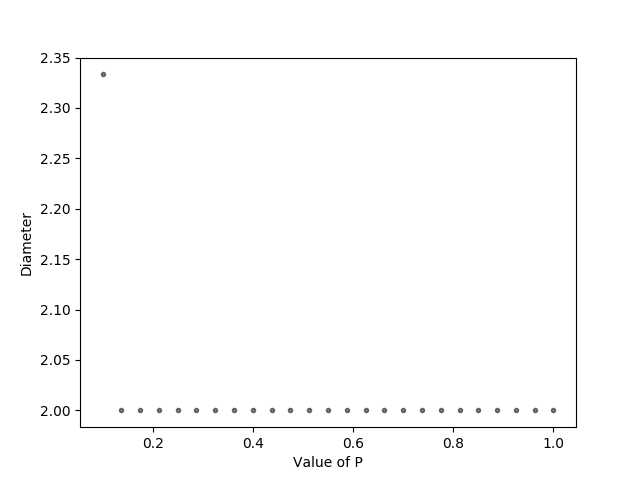
\includegraphics[width=8.4cm]{Figures/1/Diameter/m25k25num25q15.png}}
	\qquad
	\subfloat[q = 0.2]{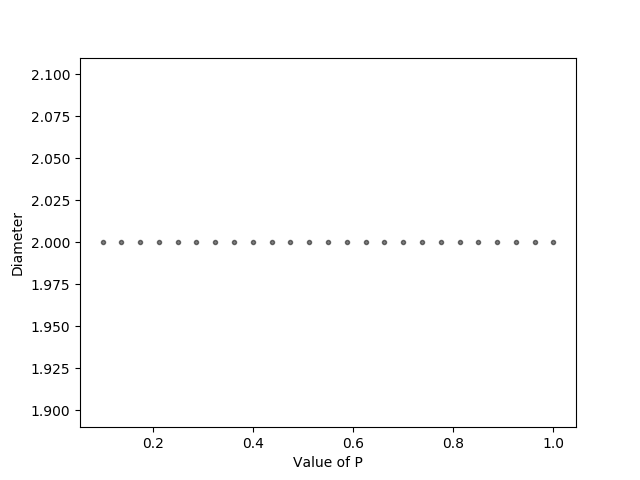
\includegraphics[width=8.4cm]{Figures/1/Diameter/m25k25num25q2.png}}
	\qquad
	\subfloat[q = 0.25]{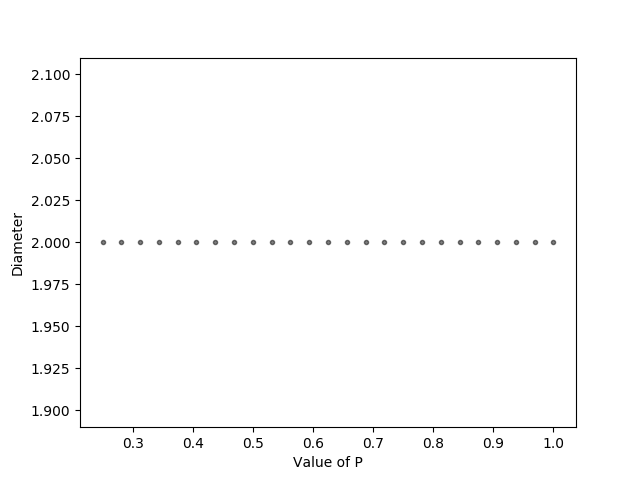
\includegraphics[width=8.4cm]{Figures/1/Diameter/m25k25num25q25.png}}
	\qquad
	\subfloat[q = 0.5]{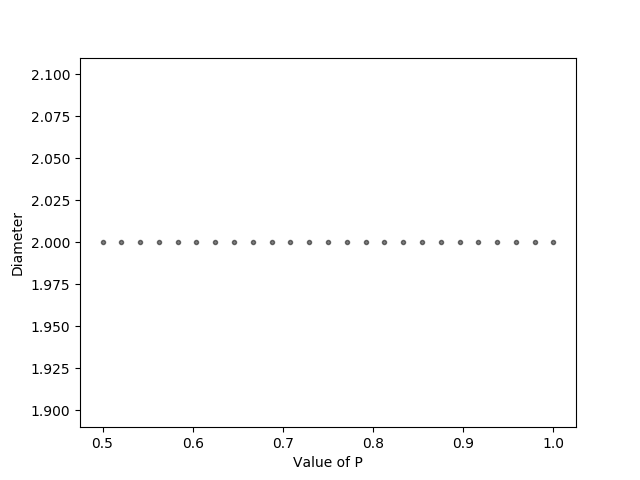
\includegraphics[width=8.4cm]{Figures/1/Diameter/m25k25num25q5.png}}
	\caption{The Diameter when varying p in a Ring Group graph for fixed q: part2}
	\label{diameters}
\end{figure*}

\newpage
\section{Question 2: Vertex Brilliance}
Parameters for Preferential Attachment (PA) Graphs and Ring Group (RG) Graphs were established by trial and error until similar numbers of vertices and edges were achieved to that of the co-authorship graph example, with 1559 vertices and 40016 edges respectively. For PA graphs, the number of vertices was set to 1559 to exactly match. PA Graphs are generated initially directed and is subsequently converted so edges are undirected. An approximate out degree of 35 for generation achieved on average 39610 over 100 samples compared with 41497 for out degree 36. Therefore, the out degree is valued at 35 to achieve similarity with co-authorship. For the plotting and analysis of PA graphs and RG graphs, data was averaged over 100 samples.

\begin{table}[h]
	\begin{tabular}{lccccc}
		\multicolumn{3}{l}{}                                                                                                                                          & \multicolumn{3}{c}{\textbf{Brilliance Distribution}} \\ \cline{2-6} 
		\multicolumn{1}{l|}{}                             & \multicolumn{1}{c|}{{\ul \textbf{Number of Nodes}}} & \multicolumn{1}{c|}{{\ul \textbf{Number of Edges}}} & \multicolumn{1}{c|}{\textbf{Mean}} & \multicolumn{1}{c|}{\textbf{Variance}} & \multicolumn{1}{c|}{\textbf{Range}} \\ \hline
		\multicolumn{1}{|l|}{\textbf{Coauthorship Graph}} & \multicolumn{1}{c|}{1559}                           & \multicolumn{1}{c|}{40016}                          & \multicolumn{1}{c|}{16.260}        & \multicolumn{1}{c|}{239.508}           & \multicolumn{1}{c|}{122}            \\ \hline
		\multicolumn{1}{|l|}{\textbf{PA Graph}}           & \multicolumn{1}{c|}{1559}                           & \multicolumn{1}{c|}{39622.0}                        & \multicolumn{1}{c|}{29.762}        & \multicolumn{1}{c|}{12.027}            & \multicolumn{1}{c|}{22}             \\ \hline
		\multicolumn{1}{|l|}{\textbf{Ring Group Graph}}   & \multicolumn{1}{c|}{1550}                           & \multicolumn{1}{c|}{39519.0}                        & \multicolumn{1}{c|}{29.728}        & \multicolumn{1}{c|}{12.427}            & \multicolumn{1}{c|}{22}             \\ \hline
	\end{tabular}
\end{table}

\subsection{Co-authorship graph}
\begin{figure*}[h]
	\centering
	\subfloat[Distribution]{{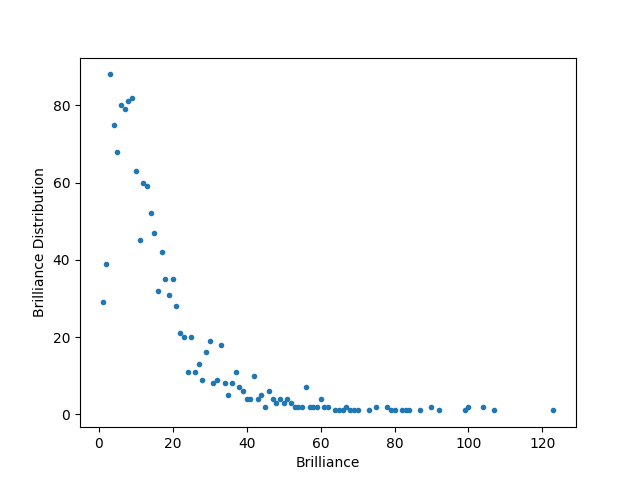
\includegraphics[width=8.4cm]{Figures/2/coauthorship.png} }}
	\qquad
	\subfloat[logplot]{{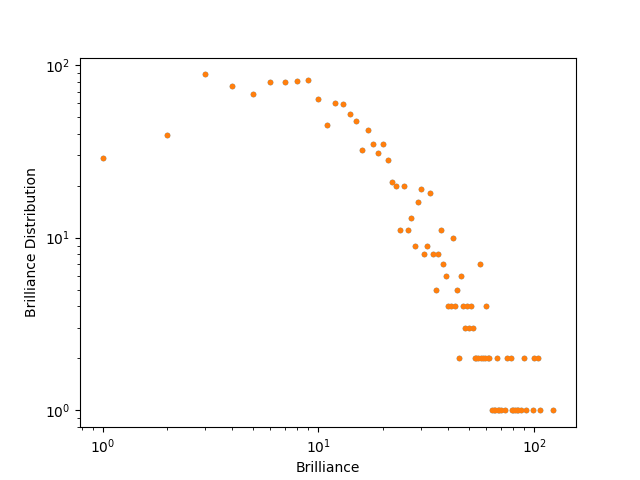
\includegraphics[width=8.4cm]{Figures/2/coauthorshiplogplot.png} }}
	\caption{Co-Authorship Brilliance distribution}
	\label{both}
\end{figure*}

The graph seems to resemble an inverse Gaussian distribution. A normal Gaussian distribution would be present if the data was random and the skewed results indicate a pattern. A peak at early brilliance can potentially be explained by suggesting academics co-author each others work in small groups, separated by topic/genre, co-authoring similar topics amongst devisable groups. As such academics are likely to cluster amongst themselves. Since work is usually very specific, academics will commonly only reference a select few other academics and vice versa, given that there is a limited amount of research in a particular area. This will lead to natural clusters forming in the data, grouping academics together where they work on similar topic areas. Graphically, this means that such groups with see high connectivity amongst themselves with infrequent adjacency to other parts of the graph. As a result, the brilliance of such groups will reflect their size, given that they are connected to each other and as such more vertices must be removed before a k-star is created. The peak at the start of the graph reflects this, showing a average size of these clusters reflected in the brilliance. The distribution then declines as we move away to more infrequent cluster sizes. Such conclusions though are limited by the breadth of the data, however the significant difference in the mean and significantly higher variance of plots when compared to the other graphs indicates clustering maybe taking place, therefore explaining the resulting brilliance distribution.
  
\subsection{PA Graphs}
\begin{figure*}[h]
	\centering
	\subfloat[Distribution]{{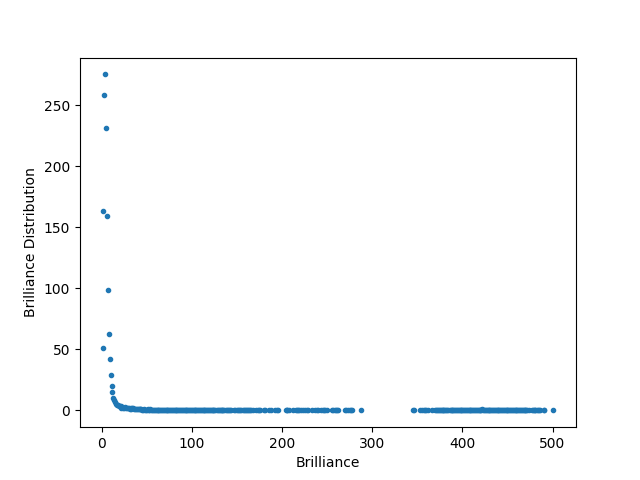
\includegraphics[width=8.4cm]{Figures/2/pagraphnumNodes.png} }}
	\qquad
	\subfloat[logplot]{{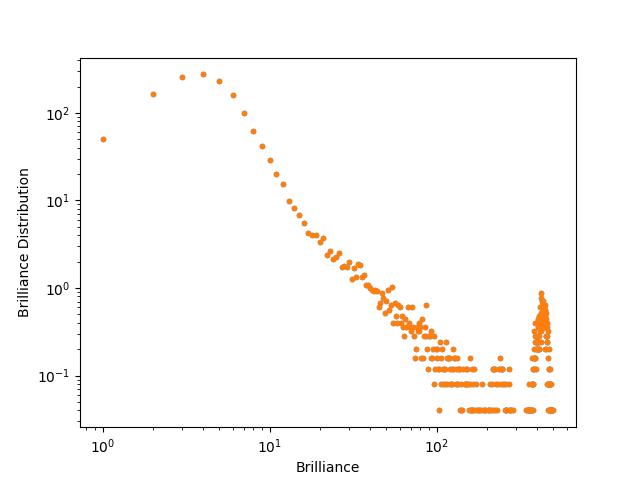
\includegraphics[width=8.4cm]{Figures/2/pagraphnumNodeslopplot.png} }}
	\caption{PA Graph Brilliance distribution, numberOfNodes=1559, outDegree=35}
	\label{both}
\end{figure*}
The chosen method for generating PA graphs was to produce a directed graph using the out-degree and number of nodes as parameters and then converting the result into an undirected representation.

The resulting plot is heavily skewed, with smaller brilliance values frequently appearing and then less brilliance variation looking towards the end. When the first few vertices are allocated edges, they are done so to every other vertex in the graph. The number of such vertices is equal to the out degree and such nodes have a maximum vertex degree. This means a star graph with them at the centre is the same graph and as such, a maximal independent set and thus vertex brilliance created is very high due to the amount of options for removal available. As more vertices are established, the degree of each steadily decreases and with it the vertex brilliance. This yields the trend seen in figure 10(a) until a stability point is reached whereby the degree will not decrease any further. This explains the spike at the start of the graph. 

\subsection{Ring Group Graphs}
\begin{figure*}[h]
	\centering
	\subfloat[Distribution]{{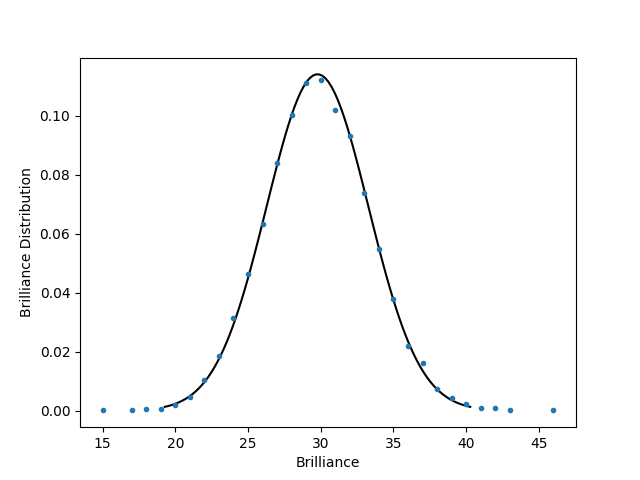
\includegraphics[width=8.4cm]{Figures/2/ring_group_graphnormalized.png} }}
	\qquad
	\subfloat[logplot]{{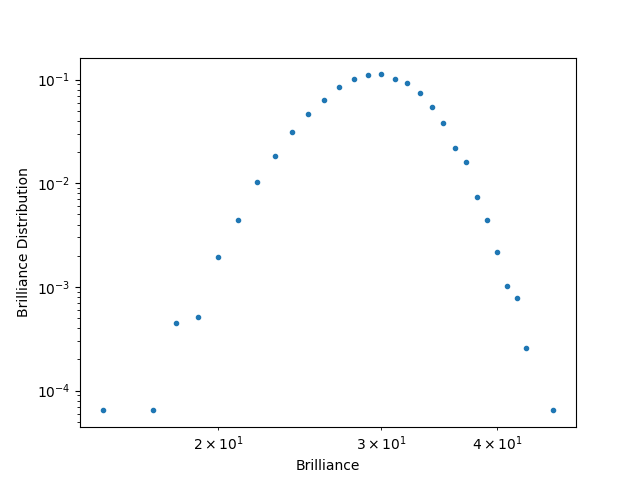
\includegraphics[width=8.4cm]{Figures/2/ring_group_graphlogplot.png} }}
	\caption{RG Graph Brilliance distribution m=50, k=31 p=0.08, q=0.03}
	\label{both}
\end{figure*}

The chosen graph size is m=50 k=31 (1550 nodes in total), p=0.08 and q=0.03. The brilliance distribution, like the degree distribution in section 1, seems to follow a binomial distribution. Approximating to the normal distribution and plotting the expected results shows that this connection. Because of the link between the degree distribution and vertex brilliance, with a higher degree lending its self towards a higher potential independent set and subsequently a higher brilliance value, the brilliance trend is pretty much identical to that of degree distribution. Figure 10(a) shows this, with a normal distribution plotted on normalized brilliance results to show the similarity.

\newpage
\section{Question 3: Graph Searching}
During graph searching, the next node queried should have the highest probability of being the target vertex compared to every other vertex in the graph. The algorithm searching the graph should follow this procedure in order to minimise the amount of queries made and the resulting search time.

\subsection{Random Graphs}
A random graph is generated by specifying the number of nodes in the graph, n followed by a probability, p that each vertex is connected to another vertex. When searching a random graph, there are multiple potential strategies to consider:

\begin{enumerate}
	\item Query all neighbours of a vertex searching for the target vertex. If not found move to a random new node
	\item Partially query the neighbours of the current vertex, only analysing a selected few, decided upon by the algorithm, succeeding if the target vertex is found and if not moving to one of the queried nodes. The percentage queried is the equal to the number of neighbours times the probability used to generate the random graph.
	\item Randomly pick a vertex from the list of a neighbours, finishing if it is the target vertex else moving to it and repeating. This is equivalent to a random walk.

\end{enumerate}

\begin{algorithm}
	\caption{Query All: Random Graph Searching Algorithm}\label{random}
	\begin{algorithmic}[1]
		\Require{$ Graph, startVertex, targetVertex$} 
		\State {$searchTime$ $\gets$ {$0$}}
		\State {$neighbours$ $\gets$ {$graph[currentVertex]$}}
		\While {$Target Vertex Not Found}$
		\State {$currentVertex$ $\gets$ {$startVertex$}}
		\For{$ \textit{neighbour in neighbours}$} \Comment{$\textit{Loop through all neighbours of the current vertex}$}
		\State {$searchTime$ $\gets$ {$searchTime + 1$}}
		\EndFor
		\If {$neighbour == targetVertex $} \Return $\textit{searchTime}$ \\\Comment{$\textit{Return search time if target found}$}
		\EndIf
		\State $\textit{currentVertex} \gets \textit{random neighbour}$ \Comment{$\textit{Else randomly move to a new vertex}$}
		\EndWhile\label{while}
	\end{algorithmic}
\end{algorithm}

Each of these strategies was attempted, however method 1 is optimal. As already stated, the query made should be on the vertex in the graph that currently has the highest probability of being the target vertex.

In a random graph, every vertex has an equal chance of being adjacent to the target vertex, with probability p. The total number of other vertices in the graph is equal to (n-1) and the expected degree therefore for the current vertex is p(n-1). Therefore:

\begin{align*}
	\text{Probability that a given vertex is connected to the target} = \frac{p}{p(n-1)} = \frac{1}{(n-1)}
\end{align*} 

The initial query therefore has probability $\frac{1}{n-1}$ of being the target vertex. However, after a query has been made to a neighbour, that vertex is confirmed as not being the target, therefore the total sample space decreases in size by 1. The probability that a query to a second neighbour being the target vertex is $\frac{1}{n-2}$. The probability of finding the target therefore increases as you query more neighbours following the formula $\frac{1}{n-i}$ where i is the query number.

This means that for a random graph, independent of the probability p, used to generate the graph, querying all the neighbours will on average yield the best search time.

For data analysis, 100,000 graph samples were taken and averaged, with the search times measured and plotted. 100 vertices were used in the graph, in order to narrow down the possible search times and improve the resulting plot. Two probabilities were analysed, 0.5 and 0.25. The data shows that querying all the neighbours yields the lowest variance/spread in search times and on average will find the target vertex fastest according to the mean.
 \newpage
  \begin{figure*}[h]
 	\centering
 	\subfloat[Query All]{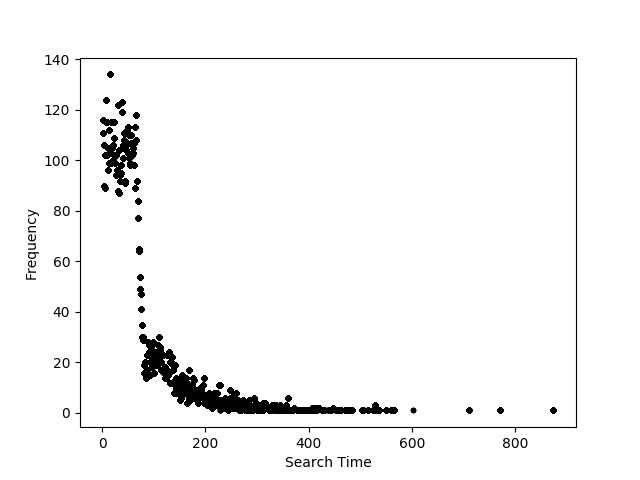
\includegraphics[width=8.4cm]{Figures/3/Random/All05.png}}
 	\qquad
 	\subfloat[Partial Query]{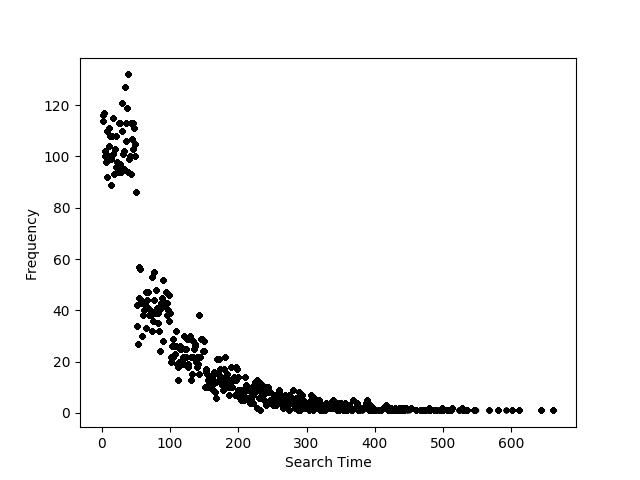
\includegraphics[width=8.4cm]{Figures/3/Random/Relative05.png}}
 	\qquad
 	\subfloat[Random Walk]{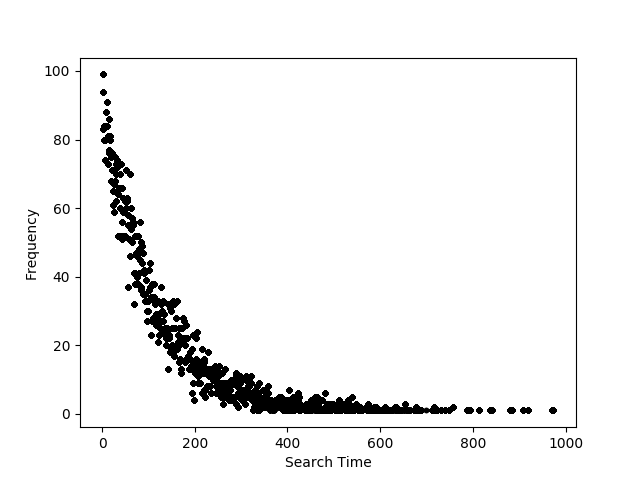
\includegraphics[width=8.4cm]{Figures/3/Random/One05.png}}		
	\caption{Random graph, p = 0.5}
 	\label{both}
 \end{figure*}

\vspace{30mm}

\begin{table}[h]
	\centering
	\begin{tabular}{lccc}
		& \multicolumn{3}{c}{{\ul \textbf{Search Time}}}                                                                    \\ \cline{2-4} 
		\multicolumn{1}{l|}{}                               & \multicolumn{1}{c|}{\textbf{Mean}} & \multicolumn{1}{c|}{\textbf{Variance}} & \multicolumn{1}{c|}{\textbf{Range}} \\ \hline
		\multicolumn{1}{|l|}{\textbf{Query All Neighbours}} & \multicolumn{1}{c|}{78.437}        & \multicolumn{1}{c|}{5648.181}          & \multicolumn{1}{c|}{822}            \\ \hline
		\multicolumn{1}{|l|}{\textbf{Partial Querying}}     & \multicolumn{1}{c|}{83.892}        & \multicolumn{1}{c|}{7238.326}          & \multicolumn{1}{c|}{954}            \\ \hline
		\multicolumn{1}{|l|}{\textbf{Random Walk}}          & \multicolumn{1}{c|}{111.768}       & \multicolumn{1}{c|}{13036.946}         & \multicolumn{1}{c|}{989}            \\ \hline
	\end{tabular}
	\caption{Random graph, p = 0.5}
\end{table}

\newpage
 \begin{figure*}[h]
	\centering
	\subfloat[Query All]{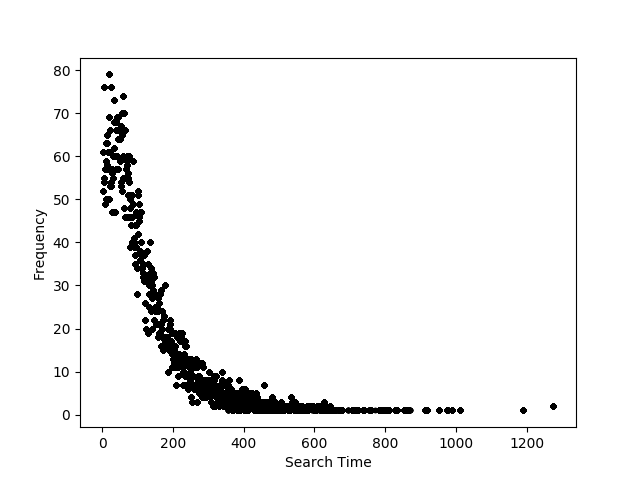
\includegraphics[width=8.4cm]{Figures/3/Random/All025.png}}
	\qquad
	\subfloat[Partial Query]{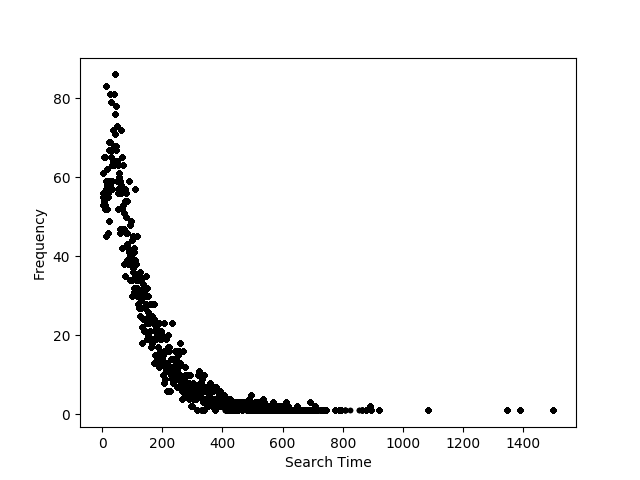
\includegraphics[width=8.4cm]{Figures/3/Random/Relative025.png}}
	\qquad
	\subfloat[Random Walk]{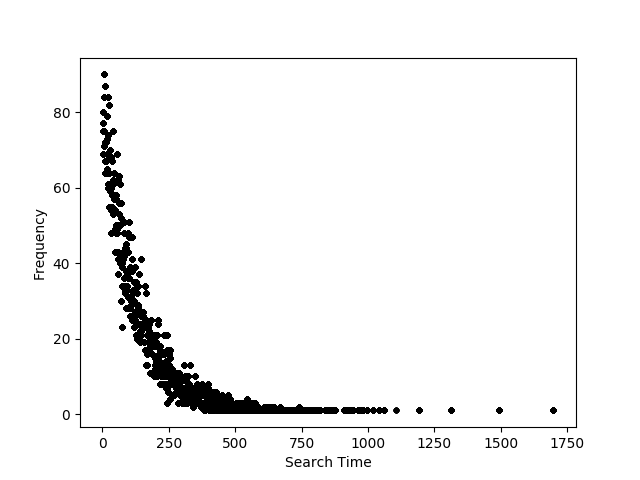
\includegraphics[width=8.4cm]{Figures/3/Random/One025.png}}		
	\caption{Random graph, p = 0.25}
	\label{both}
\end{figure*}

\vspace{30mm}

\begin{table}[h]
	\centering
	\begin{tabular}{lccc}
		& \multicolumn{3}{c}{{\ul \textbf{Search Time}}}                                                                    \\ \cline{2-4} 
		\multicolumn{1}{l|}{}                               & \multicolumn{1}{c|}{\textbf{Mean}} & \multicolumn{1}{c|}{\textbf{Variance}} & \multicolumn{1}{c|}{\textbf{Range}} \\ \hline
		\multicolumn{1}{|l|}{\textbf{Query All Neighbours}} & \multicolumn{1}{c|}{68.513}        & \multicolumn{1}{c|}{4462.571}          & \multicolumn{1}{c|}{832}            \\ \hline
		\multicolumn{1}{|l|}{\textbf{Partial Querying}}     & \multicolumn{1}{c|}{72.729}        & \multicolumn{1}{c|}{5341.012}          & \multicolumn{1}{c|}{903}            \\ \hline
		\multicolumn{1}{|l|}{\textbf{Random Walk}}          & \multicolumn{1}{c|}{83.752}        & \multicolumn{1}{c|}{7124.257}          & \multicolumn{1}{c|}{864}            \\ \hline
	\end{tabular}
	\caption{Random graph, p = 0.25}
\end{table}

\newpage
\subsection{Ring Group Graphs}
Due to the structure of a ring group graph relative to that of a random graph, searching is more complex but heuristics can be used to reduce the search time. p > q, meaning nodes in the same or adjacent group to the target vertex are more likely to be connected. For the purposes of this report, 3 algorithms were created and compared between each other.

\vspace{10mm}

\begin{enumerate}
	\item Query All: As above query every vertex and if the target is not found move to a random vertex.
	\item Group Hierarchy: Create a list of all possible groups in the graph, ordered by preference. The preference will attempt to maximise the chance that the next vertex moved to is adjacent to the target vertex by either moving to the relevant adjacent/specific group or moving in an either clockwise or counter-clockwise direction round the ring so as to move closer to the target group and increase the probability of finding the target vertex.  
	\item Partial Querying: This method is intelligent and similar to the previous. However, it utilises a random walk, hoping to find a group adjacent to or containing the target vertex by chance. If adjacent to or in the same group, it queries all neighbours looking for the target, however if not, it randomly moves to another neighbour and avoids wasting search time by querying all nodes to look for a closer option.
\end{enumerate}

\algdef{SE}[SUBALG]{Indent}{EndIndent}{}{\algorithmicend\ }%
\algtext*{Indent}
\algtext*{EndIndent}

\begin{algorithm}
	\caption{Group Hierarchy Searching Algorithm}\label{group}
	\begin{algorithmic}[1]
		\Require{$ Graph, m, k, startVertex, targetVertex$} 
		\State {$searchTime$ $\gets$ {$0$}}
		\State {$startGroup$ $\gets$ {$\textit{get startVertex Group}$}}  \Comment{$\textit{Function gets the group of a vertex}$}
		\State {$targetGroup$ $\gets$ {$\textit{get targetVertex Group}$}}
		\State {$currentVertex$ $\gets$ {$startVertex$}} 
		\\
		\State {$orderedGroups$ $\gets$ {$groupPriority(m, k, startGroup, targetGroup)$}} \\
		 \Comment{$\textit{List specifying preference for groups. Takes into account direction around the ring}$}
		\\
		\While {$Target Vertex Not Found}$
		\State {$neighbours$ $\gets$ {$graph[currentVertex]$}} 		 \Comment{$\textit{The order of vertices in neighbours is random}$}
		\State {$oldGroup$ $\gets$ {$startVertex$}} 
		\State {$bestGroupFound$ $\gets$ {$\textit{lowest ranked group}$}} 
		\For{$ \textit{neighbour in neighbours}$} \Comment{$\textit{Loop through all neighbours of the current vertex}$}
		\State {$searchTime$ $\gets$ {$searchTime + 1$}}
		\If {$neighbour == targetVertex $} \Return searchTime 
		\Else	\Comment{$\textit{Return search time if target found}$}
		\State {$neighbourGroup$ $\gets$ {$groupNumber(targetVertex, k)$}}
		\If {$ \textit{oldGroup != neighbourGroup and ranked(bestGroupFound) < ranked(group)} $} 
			\State {$bestGroupFound$ $\gets$ {$neighbourGroup$}}
			\State {$currentVertex$ $\gets$ {$neighbour$}}
		\If {$ \textit{bestGroupFound equal to or adjacent to the targetGroup}$}
			\State {$\textit{Break}$}
		\EndIf
		\EndIf
		\EndIf
		\EndFor
		
		\EndWhile\label{while}
	\end{algorithmic}
\end{algorithm}

\begin{algorithm}
	\caption{Partial Querying Searching Algorithm}\label{partial}
	\begin{algorithmic}[1]
		\Require{$ Graph, m, k, p, q, startVertex, targetVertex$} 
		\State {$searchTime$ $\gets$ {$0$}}
		\State {$targetGroup$ $\gets$ {$get targetVertex Group$}}
		\State {$highGroups$ $\gets$ {$\textit{Target group and 2 adjacent groups}$}}
		\State {$vertexChanged$ $\gets$ {$\textit{False}$}}
		\\
		\While {$Target Vertex Not Found}$
		\State {$currentGroup$ $\gets$ {$\textit{get currentVertex Group}$}}
		\State {$neighbours$ $\gets$ {$graph[currentVertex]$}} 		 \Comment{$\textit{The order of vertices in neighbours is random}$}
		
		\If {$ \textit{group(currentVertex) in highGroups)}$}
		\For{$ \textit{neighbour in neighbours}$}
		\State {$neighbourGroup$ $\gets$ {$get neighbour Group$}}
		\State {$searchTime$ $\gets$ {$searchTime + 1$}}
		\If {$neighbour == targetVertex $} \Return $\textit{searchTime}$
		\EndIf
		\If {$\textit{neighbourGroup in highGroups}$} 
		\State {$currentVertex$ $\gets$ {$neighbour$}}
		\State {$vertexChanged$ $\gets$ {$\textit{True}$}}
		\EndIf
		\EndFor
		
		\If {$\textit{vertexChanged}$} \Comment{$\textit{If a vertex from the high group was not found}$}
			\State {$currentVertex$ $\gets$ {$\textit{random neighbour}$}}
		\EndIf
		\Else
		\State {$searchTime$ $\gets$ {$searchTime + 1$}}
		\State {$currentVertex$ $\gets$ {$\textit{random neighbour}$}}
		\EndIf
		\EndWhile\label{while}
	\end{algorithmic}
\end{algorithm}

The group hierarchy algorithm was the first that came to mind. The idea behind the implementation was that it is desirable to move as close to the target group and its adjacent groups as possible, as these vertices have a probability p of being adjacent to the target. Therefore, the algorithm ranks each of the groups in terms of its 'desirability', that in the immediate future, entering that group will yield a higher probability of finding the target vertex. If the current vertex is not adjacent to another vertex in the target group, then it should move to the groups adjacent to the target. If neither of these are possible, moving to another group is an option, ideally as close to the desirable groups as possible. Because of adjacency between groups, moving around the ring is possible for when the value of q is really low. In this case, one wants to move either clockwise or anti-clockwise round the ring depending on which route is shortest. This is what the group hierarchy decides. Once in the group or those adjacent, the algorithm stays inside the 3 groups because it is here that the highest chance of finding the target exists. The algorithm is therefore very good if presented with a relatively sparse ring graph with lots of small groups as it can effectively navigate between them. The issue with this implementation is the almost unnecessary checking of every neighbour, which is very heavy on the search time. When there is a low probability of finding the target, there is little reason to check every neighbour but the algorithm still has to in order to find the best possible group it can advance to next.

This is what inspired the Partial Querying algorithm. The algorithm follows much the same logic as group hierarchy except it only pays attention to the target group and those adjacent to it. At a vertex, if it is not in the same or adjacent group to the target, the algorithm will simply randomly choose a neighbour to move to recursively. If the group is correct, every neighbour will be queried looking for the target. If it is not found, another vertex adjacent to the current one will be moved to as long as it is in the same or adjacent group.

The two algorithms balance between them querying more often for more intelligent decision making, with spontaneous choice. Experiments were conducted on the a Ring Group Graph with parameters: m=k=10, p=0.4 and q=0.1. The sample size for calculation was 100,000 with the final results representing an average over each.

\begin{figure*}[h]
	\centering
	\subfloat[Query All]{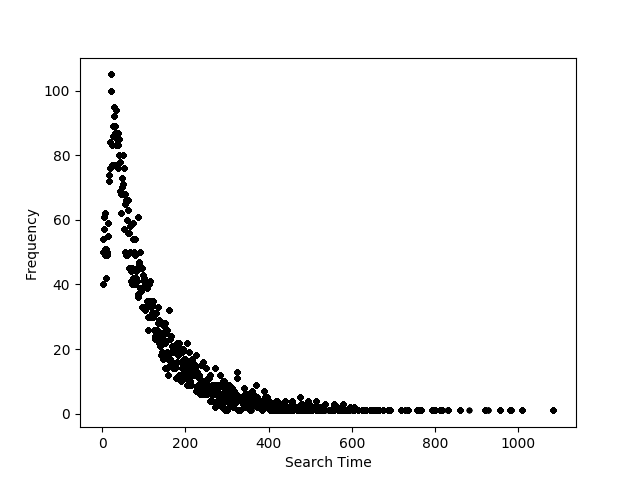
\includegraphics[width=8.4cm]{Figures/3/Ring/randomp04.png}}
	\qquad
	\subfloat[Group Hierarchy Algorithm]{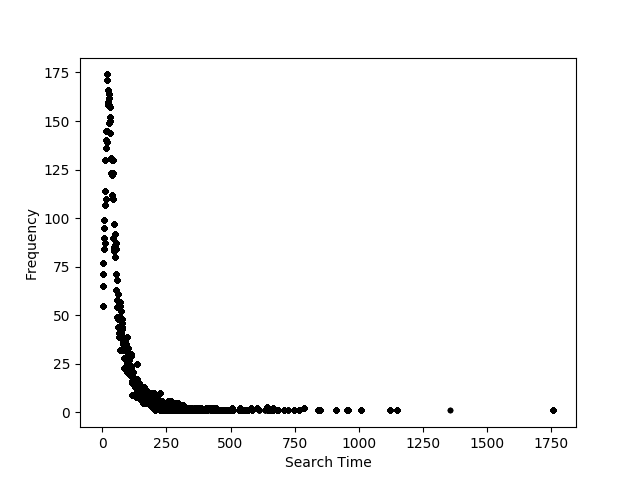
\includegraphics[width=8.4cm]{Figures/3/Ring/groupp04.png}}
	\qquad
	\subfloat[Partial Query Algorithm]{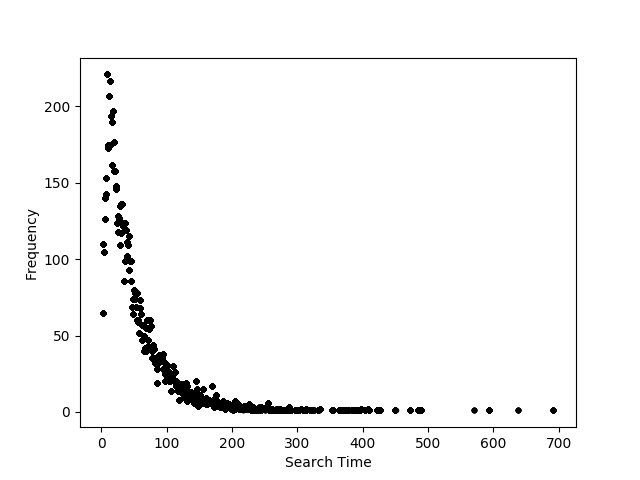
\includegraphics[width=8.4cm]{Figures/3/Ring/partialp04.png}}		
	\caption{Ring Group Graph: m=k=10, p=0.4, q=0.1}
	\label{both}
\end{figure*}

\vspace{100 mm}


\begin{table}[h]
	\centering
	\begin{tabular}{lccc}
		& \multicolumn{3}{c}{{\ul \textbf{Search Time}}}                                                                    \\ \cline{2-4} 
		\multicolumn{1}{l|}{}                         & \multicolumn{1}{c|}{\textbf{Mean}} & \multicolumn{1}{c|}{\textbf{Variance}} & \multicolumn{1}{c|}{\textbf{Range}} \\ \hline
		\multicolumn{1}{|l|}{\textbf{Query All}}      & \multicolumn{1}{c|}{111.018}       & \multicolumn{1}{c|}{13211.223}         & \multicolumn{1}{c|}{1770}           \\ \hline
		\multicolumn{1}{|l|}{\textbf{Group Hierarchy}} & \multicolumn{1}{c|}{57.927}        & \multicolumn{1}{c|}{6744.383}          & \multicolumn{1}{c|}{1758}           \\ \hline
		\multicolumn{1}{|l|}{\textbf{Partial Query}}  & \multicolumn{1}{c|}{41.616}        & \multicolumn{1}{c|}{2980.924}          & \multicolumn{1}{c|}{1639}           \\ \hline
	\end{tabular}
	\caption{Ring Group Graph: m=k=10, p=0.4, q=0.1}
\end{table}

\newpage 
 
Interestingly, the partial query algorithm was much more consistent at producing better results according to table 4. It yielded the lowest variance quite significantly and as can be seen in figure 14(c), and the lowest max search time. In comparison, group hierarchy has the highest maximum search time even when compared to a random query all strategy. The mean search time is lowest for partial query consistently but is closely followed by group hierarchy. Further tests would be required, experimenting with values of m,k,p and q to vary the graph structure and see which copes best. However, under the tests done here partial query has the lowest max search time, mean and variance between searches so is the logical choice for the search algorithm.

An additional feature was also added in latter stages of development, nicknamed the 'break chance'. In the incredibly unlikely possibility that either algorithm gets caught in a loop between the vertices in a group that are not directly connected to the target vertex (in the event of much lower p values), the algorithm will move to a random neighbour under a certain probability, currently set to:

\begin{align*}
	Break Chance = c \cdot{}\frac{q}{pmk}  \textit{ where c is some constant}
\end{align*}

The rationale behind this is that for high values of q, the chances increase and if for higher values of any other parameter they decrease. High values of p mean the probability, if in the same group, target are higher. Likewise, for larger values of k, there are more vertices that have a chance of being adjacent to the target. High values of m mean more groups so if leaving the target room is will be harder to return. The break chance technique was experimented with and included for completeness but is only necessary for more extreme parameters. Break chance was implemented to prevent looping in experimenting sample sizes over 1 million where it could occur. 

\end{document}